\documentclass{tarea}


\renewcommand{\hmwkTitle}{Guía 01: Modelos Matemáticos}
\renewcommand{\hmwkDueDate}{08 de Febrero de 2017}
\renewcommand{\hmwkClass}{Investigación Operativa}
\renewcommand{\hmwkClassInstructor}{C.C. Lauritto \& Ing. Casanova}
\renewcommand{\hmwkAuthorName}{\textbf{ Ravera P. \& Rivera R.}}

\begin{document}

\caratula
\tableofcontents
\pagebreak

\section{Ejercicios}
\begin{homeworkProblem}

\begin{itemize}
\item {\bfseries Modelo a: }Determinístico, lineal y continuo
\item {\bfseries Modelo b: }Determinístico, lineal y continuo
\item {\bfseries Modelo c: }Determinístico, lineal y entero
\item {\bfseries Modelo d: }Determinístico, no lineal y restringido
\item {\bfseries Modelo e: }Determinístico, no lineal y restringido
\item {\bfseries Modelo f: }Determinístico, no lineal y restringido
\item {\bfseries Modelo g: }Determinístico, lineal y mixto (entero y binario)
\end{itemize}
\end{homeworkProblem}
\pagebreak

\section{Modelado de Problemas}
\begin{homeworkProblem}[1][Destilación de Crudos]
\begin{align*}
Min\ Z &	= 4G + 6P + 7S \\
&s.a. \\
C_1 &\le 1400 \\
C_2 &\le 2000 \\
G &\ge 900 \\
P &\ge 300 \\
S &\ge 800 \\
S &\le 1700 \\
\end{align*}
\end{homeworkProblem}


\begin{homeworkProblem}[-1][Televisores]
Siendo $x$ la cantidad de televisores de 27'' e $y$ la cantidad de televisores de 20'' a producir, entonces debemos minimizar la función\\
\begin{equation}
Max\ Z=120\fraccorche{\$}{Ux} x\corche{Ux} +80\fraccorche{\$}{Uy}y\corche{Uy} 
\end{equation}
sujeta a las siguientes restricciones:
\begin{align*}
x  \corche{Ux } & \le 40\corche\{*\} \\
y\corche{Uy} & \le 10\corche\{(1)\} \\
20\fraccorche{Hs}{Ux}x\corche{Ux} + 10\fraccorche{Hs}{Uy}y\corche{Uy } & \le 500\corche{Hs} \\
x,y & \ge 0
\end{align*}
Las variables de decisión son $x$ e $y$, y el modelo es determinista, lineal y entero (no debería poder producir medio televisor)
\end{homeworkProblem}

\needspace{4\baselineskip}

\begin{homeworkProblem}[-1][Transportes]
Siendo nuestras variables de decisión $A$ y $B$ representando respectivamente la cantidad de camiones de cada tipo a contratar, debemos  optimizar la función
\begin{equation}
Min\ Z= 0,30\fraccorche{\$}{Km.Ua} A\corche{Ua} + 0,40\fraccorche{\$}{Km.Ub}B\corche{Ub} 
\end{equation}
sujeta a las restricciones:
\begin{align*}
20\fraccorche{m^3\ PR}{Ua}A\corche{Ua} + 30\fraccorche{m^3\ PR}{Ub}b\corche{Ub} &\ge 900 \corche{m^3\ PR} \\
40\fraccorche{m^3\ PnR}{Ua}A\corche{Ua} + 30\fraccorche{m^3\ PnR}{Ub}b\corche{Ub} &\ge 1200 \corche{m^3\ PnR} \\
A,B &\ge 0
\end{align*}
\end{homeworkProblem}


\begin{homeworkProblem}[-1][Carnicería]
%% Table generated by Excel2LaTeX from sheet 'Simplex01'
\begin{table}[ht]
  \centering
  \caption{Add caption}
    \begin{tabular}{crr|cccccc|c}
    \hline
    \hline
           & \multicolumn{1}{c}{} & \multicolumn{1}{c}{} & $C_1$  & $C_2$  & $C_3$  & $C_4$  & $C_5$  & \multicolumn{1}{c}{$C_6$} &  \bigstrut[t]\\
    $C_k$  & \multicolumn{1}{c}{$X_k$} & \multicolumn{1}{c|}{$B_k$} & $A_1$  & $A_2$  & $A_3$  & $A_4$  & $A_5$  & $A_6$  & $\theta_i = b_i/a_ij$ \bigstrut[b]\\
    \hline
    0      & \multicolumn{1}{c}{$X_3$} & \multicolumn{1}{c|}{600} & 2      & 2      & 1      & 1      & 0      & 0      & $\theta_1 = 300$ \bigstrut\\
\cline{5-5}    0      & \multicolumn{1}{c}{\textcolor[rgb]{ 1,  0,  0}{\boldmath{}\textbf{$X_4$}\unboldmath{}}} & \multicolumn{1}{c|}{600} & \multicolumn{1}{c|}{0} & \multicolumn{1}{c|}{\textbf{4}} & 2      & 0      & 1      & 0      & \boldmath{}\textbf{$\theta_2 = 150$}\unboldmath{} \bigstrut\\
\cline{5-5}    0      & \multicolumn{1}{c}{$X_5$} & \multicolumn{1}{c|}{800} & 2      & 4      & 3      & 0      & 0      & 1      & $\theta_3 = 200$ \bigstrut\\
    \hline
    \multicolumn{3}{c|}{Z=0} & -8     & \textcolor[rgb]{ 0,  0,  1}{\textbf{-10}} & -7     & 0      & 0      & 0      &  \bigstrut\\
    \hline
    \hline
    \end{tabular}%
  \label{tab:addlabel}%
\end{table}%

Nuestras variables de decisión son la cantidad de carne de cerdo ($X_c$) y de ternera ($X_t$) por kilo de hamburguesa producida. Entonces buscamos la composición del kilo de hamburguesa que minimice el costo por kilo, definida de la siguiente forma:
\begin{equation}
Min\ Z=0,8\fraccorche{\$}{Kg_{Tern}}X_t\fraccorche{Kg_{Tern}}{Kg_{Hamb}} + 0,6\fraccorche{\$}{Kg_{Cerd}}   X_c\fraccorche{Kg_{Cerd}}{Kg_{Hamb}}
\end{equation}

y sujeta a:
\begin{align*}
0,2 \fraccorche{Kg_{Grasa}}{Kg_{Tern}} X_t\fraccorche{Kg_{Tern}}{Kg_{Hamb}} &+ 0,32\fraccorche{Kg_{Grasa}}{Kg_{Cerd}} X_c\fraccorche{Kg_{Cerd}}{Kg_{Hamb}}  \le 0,25\fraccorche{Kg_{Grasa}}{Kg_{Hamb}} \\
X_t\fraccorche{Kg_{Tern}}{Kg_{Hamb}}&+X_c\fraccorche{Kg_{Cerd}}{{Kg_{Hamb}}} = 1\corche{Kg_j} \\
X_t,X_t &\ge 0
\end{align*}

\end{homeworkProblem}


\needspace{6\baselineskip}
\begin{homeworkProblem}[-1][Compañía Minera]
En este caso, nuestras variables de decisión representan la cantidad de días que cada una de las minas debe estar operativa. 
Se busca la combinación de días que minimice el costo
\begin{equation}
Min\ Z = 2000\fraccorche{\$}{Dia_{1}}M_1\corche{Dia_{1}} + 2200\fraccorche{\$}{Dia_{2}}M_2Y\corche{Dia_{2}} + 1800\fraccorche{\$}{Dia_{3}}M_3\corche{Dia_{3}}
\end{equation}
sujeto a las restricciones:
\begin{align*}
4\fraccorche{Tn_{alta}}{Dia_1}M_1\corche{Dia_1}&+6\fraccorche{Tn_{alta}}{Dia_2}M_2\corche{Dia_2}+1\fraccorche{Tn_{alta}}{Dia_3}M_3\corche{Dia_3} = 54\corche{Tn_{alta}} \\
4\fraccorche{Tn_{baja}}{Dia_1}M_1\corche{Dia_1}&+4\fraccorche{Tn_{baja}}{Dia_2}M_2\corche{Dia_2}+6\fraccorche{Tn_{baja}}{Dia_3}M_3\corche{Dia_3} = 65\corche{Tn_{baja}} \\
M_i &\in \{0,1,2,3,4,5,6,7\}\quad \quad \forall i=1,2,3 
\end{align*}
\end{homeworkProblem}


\begin{homeworkProblem}[-1][Agropecuario]
En este problema, debemos buscar cómo distribuir nuestros cultivos en 3 fincas, de manera
de maximizar la utilidad total. Para esto trabajamos con 9 variables de decisión:
\begin{itemize}
\item $X_{1y}$ Cantidad de hectáreas de la finca 1 dedicadas a la plantación de yuca
\item $X_{1p}$ Cantidad de hectáreas de la finca 1 dedicadas a la plantación de papa
\item $X_{1m}$ Cantidad de hectáreas de la finca 1 dedicadas a la plantación de maíz
\item $X_{2y}$ Cantidad de hectáreas de la finca 2 dedicadas a la plantación de yuca
\item $X_{2p}$ Cantidad de hectáreas de la finca 2 dedicadas a la plantación de papa
\item $X_{2m}$ Cantidad de hectáreas de la finca 2 dedicadas a la plantación de maíz
\item $X_{3y}$ Cantidad de hectáreas de la finca 3 dedicadas a la plantación de yuca
\item $X_{3p}$ Cantidad de hectáreas de la finca 3 dedicadas a la plantación de papa
\item $X_{3m}$ Cantidad de hectáreas de la finca 3 dedicadas a la plantación de maíz
\end{itemize}
La utilidad total está modelada mediante la siguiente función:
\begin{align*}
Max\ Z =\quad &400\fraccorche{\$}{Ha}(X_{1y}\corche{Ha}+X_{2y}\corche{Ha}+X_{3y}\corche{Ha})\quad + \\
  &300\fraccorche{\$}{Ha}(X_{1p}\corche{Ha}+X_{2p}\corche{Ha}+X_{3p}\corche{Ha})\quad + \\
    &100\fraccorche{\$}{Ha}(X_{1m}\corche{Ha}+X_{2m}\corche{Ha}+X_{3m}\corche{Ha})
\end{align*}
la cual se halla sujeta a:
\begin{align*}
X_{1y}\corche{Ha} + X_{1p}\corche{Ha} + X_{1m}\corche{Ha} &\le 350\corche{Ha} \\
X_{2y}\corche{Ha} + X_{2p}\corche{Ha} + X_{2m}\corche{Ha} &\le 700\corche{Ha} \\
X_{3y}\corche{Ha} + X_{3p}\corche{Ha} + X_{3m}\corche{Ha} &\le 300\corche{Ha} \\
\\
5\fraccorche{Agua}{Ha}X_{1y}\corche{Ha} + 4\fraccorche{Agua}{Ha}X_{1p}\corche{Ha} + 3\fraccorche{Agua}{Ha}X_{1m}\corche{Ha} &\le 1500\corche{Agua} \\
5\fraccorche{Agua}{Ha}X_{2y}\corche{Ha} + 4\fraccorche{Agua}{Ha}X_{2p}\corche{Ha} + 3\fraccorche{Agua}{Ha}X_{2m}\corche{Ha} &\le 2000\corche{Agua} \\
5\fraccorche{Agua}{Ha}X_{3y}\corche{Ha} + 4\fraccorche{Agua}{Ha}X_{3p}\corche{Ha} + 3\fraccorche{Agua}{Ha}X_{3m}\corche{Ha} &\le 900\corche{Agua} \\
\\
X_{1y}\corche{Ha} + X_{2y}\corche{Ha} + X_{3y}\corche{Ha} &\le 1500\corche{Ha} \\
X_{1p}\corche{Ha} + X_{2p}\corche{Ha} + X_{3p}\corche{Ha} &\le 2000\corche{Ha} \\
X_{1m}\corche{Ha} + X_{2m}\corche{Ha} + X_{3m}\corche{Ha} &\le 900\corche{Ha} \\
\end{align*}
\begin{align*}
\frac{X_{1y}\corche{Ha} + X_{1p}\corche{Ha} + X_{1m}\corche{Ha}}{350\corche{Ha}} &= \frac{X_{2y}\corche{Ha} + X_{2p}\corche{Ha} + X_{2m}\corche{Ha}}{700\corche{Ha}}\\
\frac{X_{1y}\corche{Ha} + X_{1p}\corche{Ha} + X_{1m}\corche{Ha}}{350\corche{Ha}} &= \frac{X_{3y}\corche{Ha} + X_{3p}\corche{Ha} + X_{3m}\corche{Ha}}{300\corche{Ha}}\\
\frac{X_{2y}\corche{Ha} + X_{2p}\corche{Ha} + X_{2m}\corche{Ha}}{700\corche{Ha}} &= \frac{X_{3y}\corche{Ha} + X_{3p}\corche{Ha} + X_{3m}\corche{Ha}}{300\corche{Ha}}
\end{align*}
\end{homeworkProblem}


\begin{homeworkProblem}[-1][Ómnibus]
Debemos decidir cuántos choferes contratar y despedir por año, a fin de minimizar el costo del personal, siempre satisfaciendo el nivel operativo mínimo.
Las variables de decisión son:
\begin{itemize}
\item $C_i$: Cantidad de choferes contratados en el año $i$
\item $D_i$: Cantidad de choferes despedidos en el año $i$
\end{itemize}
La función de costo es:
\begin{align*}
Min\ Z = 10000\fraccorche{\$}{Ch}\left(50 + \sum_{i=1}^{5}{\sum_{j=1}^{i}{C_j-D_j}}\right)\corche{Ch} \\
+ 4000\fraccorche{\$}{Ch}\sum_{i=1}^{5}{C_i}\corche{Ch} + 2000\fraccorche{\$}{Ch}\sum_{i=1}^{5}{D_i}\corche{Ch}
\end{align*}
sujeta a
\begin{align*}
\text{Siendo: } choferes = \corche{60, 70, 50,65,75} \text{un vector.}\\
\forall i=1...5\quad \corche{50 + \left(\sum_{j=1}^{i-1}{C_j-D_j} \right) + C_i - D_i}\corche{Ch} = choferes_i\corche{Ch} \\
\forall i=1...5\quad C_i,D_i \in \mathbb{Z}
\end{align*}
\end{homeworkProblem}


\begin{homeworkProblem}[-1][Mainframe Seguridad]
Se busca minimizar el costo de realizar backups de las bases de datos de un Mainframe, el cual es proporcional a la cantidad de GB utilizados.
Contamos con 10 cintas de distintas capacidades, siendo el siguiente el vector de costos:
\begin{align*}
capac = \corche{1.3, 5, 3.1, 4.3, 5.1, 4, 3, 1, 2, 10.2}
\end{align*}
Entonces nuestras variables de decisión tienen la forma:
\begin{itemize}
\item $X_{ij}$ Representa si a la base de datos \( i \in \left\{ A,B,C,D,E \right\}  \) se le realiza un backup en la cinta \(  j \in \left\{ 1,2,3,4,5,6,7,8,9,10 \right\} \).
\end{itemize}
Y la función de capacidades utilizadas es:
\begin{align*}
Min\ Z = \sum_{j=1}^{10}{\corche{capac_j \sum_{i=A}^{E}{X_{ij}}}}
\end{align*}
sujeta a:
\begin{align*}
X_{A3},\    X_{A6},\ &  X_{A7},\   X_{A10} = 0  \\
X_{B2},\   X_{B4},\  &X_{B5},\  X_{B7},\  X_{B8},\   X_{B9},\  X_{B10} = 0 \\
X_{C1},\   X_{C3},\  &X_{C4},\  X_{C6},\  X_{C8},\  X_{C9} =0 \\
X_{D1},\   X_{D2},\  &X_{D4},\  X_{D5},\  X_{D7},\  X_{D9},\  X_{D10} = 0 \\
X_{E3},\   X_{E5},\  &X_{E8}  = 0 \\
X_{ij} \in & \left\{  0,1 \right\}\quad\quad \forall i=A...E,j=1...10\\
\end{align*}
\end{homeworkProblem}


\begin{homeworkProblem}[-1][Monopolista]
En este caso debemos hallar el costo por producto $q$ que maximice nuestra ganancia, la cual está dada por:
\begin{equation}
  Max\ Z = \left( 100-4q-2 \right)\fraccorche{\$}{U}q\corche{U} -50\corche{\$} 
\end{equation}
Obviamente, dado que representa una cantidad, $q$ puede ser como mínimo 0 ($q \ge 0$)
\end{homeworkProblem}


\begin{homeworkProblem}[-1][Firma genérica]
Similar al caso anterior, solo que con dos mercados en los cuales vendemos nuestro producto, por lo que tendremos las variables de decisión
$q_1$ y $q_2$ que representan la cantidad vendida en cada mercado. La función a optimizar es:
\begin{equation}
  Max\ Z = 60\fraccorche{\$}{U}q_1\corche{U} + \left( 100-q_2 \right)\fraccorche{\$}{U}q_2\corche{U} - \left( q_1 + q_2 \right)^2\corche{\$}
\end{equation}
Sujeta a:
\begin{align*}
  q_1,q_2\ge 0
\end{align*}
\end{homeworkProblem}


\begin{homeworkProblem}[-1][Dos mercados]
Debemos encontrar la división del total del presupuesto de promoción, que al aplicarse nos permita maximizar el beneficio total, entonces las variables de decisión toman la forma:
\begin{itemize}
  \item $x_j$: Nivel de gasto en promocionar en el mercado $j$
\end{itemize}
La función objetivo esta dada por:
\begin{multline}
  Max\ Z = 7\fraccorche{\$}{U}6x_1^{1/2}\corche{U} - \left( 60 +24x_1^{1/2}+x_1\right)\corche{\$} \\ + 9\fraccorche{\$}{U}15x_2^{1/2}\corche{U} - \left( 28 +5x_2^{1/2}+x_2\right)\corche{\$}
\end{multline}
sujeta a:
\begin{align*}
  x_1\corche{\$} + x_2\corche{\$} = 65000\corche{\$} \\
  x_1,x_2 \ge 0
\end{align*}
\end{homeworkProblem}


\begin{homeworkProblem}[-1][Dos lámparas]
\begin{equation}
  Max\ Z = 15\fraccorche{\text{\euro}}{L1}X_1\corche{L1} +10\fraccorche{\text{\euro}}{L2}X_2{L2}
\end{equation}
\begin{align*}
  20\fraccorche{Tman}{L1}X_1{L1} + 30\fraccorche{Tman}{L2}X_2{L2} \le 6000\corche{Tman}\\
  15\fraccorche{Tmaq}{L1}X_1{L1} + 10\fraccorche{Tmaq}{L2}X_2{L2} \le 4800\corche{Tmaq}\\
  X_1,X_2 \ge 0
\end{align*}
\end{homeworkProblem}


\begin{homeworkProblem}[-1][Refinería de Petróleo]
\begin{equation}
  Min\ Z = 35\fraccorche{\$}{CL}X_L\corche{CL} + 30\fraccorche{\$}{CP}X_P\corche{CP}
\end{equation}
\begin{align*}
   0,3\fraccorche{BT}{CL}X_L\corche{CL} + 0,2\fraccorche{BT}{CP}X_P\corche{CP} \ge 500000\corche{BT} \\
 0,3\fraccorche{BG}{CL}X_L\corche{CL} + 0,3\fraccorche{BG}{CP}X_P\corche{CP} \ge 900000\corche{BG} \\
 0,2\fraccorche{BC}{CL}X_L\corche{CL} + 0,4\fraccorche{BC}{CP}X_P\corche{CP} \ge 800000\corche{BC} \\
 X_P,X_L \ge 0
\end{align*}
\end{homeworkProblem}


\begin{homeworkProblem}[-1][Dulces]
\begin{equation}
  Min\ z = 0,25\fraccorche{\$}{Kg_S}\paren{S_a + S_n + S_c}\corche{Kg_S} + 0,2\fraccorche{\$}{Kg_M}\paren{M_a+M_c+M_n}\corche{Kg_M}
\end{equation}
\begin{align*}
  S_a + S_n + S_c = 1 \\
  M_a+M_c+M_n = 1 \\
  S_n \corche{Kg_n} \ge 0,2\corche{Kg_n} \\
  M_n \corche{Kg_n} \ge 0,1\corche{Kg_n} \\
  M_c \corche{Kg_c} \ge 0,1\corche{Kg_c} \\
\end{align*}
\end{homeworkProblem}


\begin{homeworkProblem}[-1][Competencia de Veleros]
Siendo
\begin{itemize}
 \item Dorso = $\left[65,67,68,67,71,69 \right]$ los tiempos respectivos de cada nadador en el estilo Dorso
 \item Pecho = $\left[73, 70, 72, 75, 69, 71 \right]$ los tiempos respectivos de cada nadador en el estilo Pecho
 \item Marip = $\left[63,65,69,70,75,66 \right]$ los tiempos respectivos de cada nadador en el estilo Mariposa
 \item Libre = $\left[57,58,55,59,57,59 \right]$ los tiempos respectivos de cada nadador en el estilo Libre
\end{itemize}
\begin{align*}
  Min\ Z = \sum_{i=1}^{6}{X_{iD}*Dorso_i + X_{iP}*Pecho_i + X_{iM}*Marip_i + X_{iL}*Libre_i}
\end{align*}
\begin{align*}
   \sum_{i=1}{6}{X_{iD}} = 1 \\
   \sum_{i=1}{6}{X_{iP}} = 1  \\
   \sum_{i=1}{6}{X_{iM}} = 1 \\
   \sum_{i=1}{6}{X_{iL}} = 1 \\
   \forall i=1..6\quad \quad X_{iD},X_{iP},X_{iM},X_{iL} \in \{0,1\}
\end{align*}
\end{homeworkProblem}


\begin{homeworkProblem}[-1][Operario]
\begin{equation}
  Max\ Z = 100X_1 + 60X_2 + 70X_3 + 15X_4 + 15X_5
\end{equation}
\begin{align*}
  53\fraccorche{Up}{U1}X_1\corche{U1} + 23\fraccorche{Up}{U1}X_2\corche{U2} &+ 35\fraccorche{Up}{U3}X_3\corche{U3} \\
   &+ 15\fraccorche{Up}{U4}X_4\corche{U4} + 7\fraccorche{Up}{U5}X_5\corche{U5} \le 60\corche{Up} \\
  \forall i=1..5\quad \quad X_i \in \{0,1 \}
\end{align*}
\end{homeworkProblem}


\begin{homeworkProblem}[-1][Fabricante de Plástico]
\begin{multline}
  Min\ Z = 14\fraccorche{\$}{Caja}X_{11}\corche{Caja} + 13\fraccorche{\$}{Caja}X_{12}\corche{Caja} + 11\fraccorche{\$}{Caja}X_{13}\corche{Caja} + \\
  13\fraccorche{\$}{Caja}X_{21}\corche{Caja} + 13\fraccorche{\$}{Caja}X_{22}\corche{Caja} + 12\fraccorche{\$}{Caja}X_{23}\corche{Caja} 
\end{multline}
\begin{align*}
  X_{11}\corche{Caja} + X_{12}\corche{Caja} + X_{13}\corche{Caja} \le   1200\corche{Caja}\\
  X_{21}\corche{Caja} + X_{22}\corche{Caja} + X_{23}\corche{Caja} \le   1000\corche{Caja}\\
  X_{11}\corche{Caja} + X_{21}\corche{Caja}  \le 1000 \corche{Caja} \\
  X_{12}\corche{Caja} + X_{22}\corche{Caja}  \le 700 \corche{Caja}\\
  X_{13}\corche{Caja} + X_{23}\corche{Caja}  \le 500 \corche{Caja}\\
    \forall i=1..2\ ,\ j=1..3\quad \quad X_{ij} \in \{0,1 \}
\end{align*}
\end{homeworkProblem}


\begin{homeworkProblem}[-1][MG Auto]
\begin{multline}
  Max\ Z = \paren{80 \times 1000}\fraccorche{\$}{Auto}X_{11}\corche{Auto} +
           \paren{125 \times 2690}\fraccorche{\$}{Auto}X_{12}\corche{Auto} + \\
           \paren{125 \times 1000}\fraccorche{\$}{Auto}X_{21}\corche{Auto} + 
           \paren{108 \times 1350}\fraccorche{\$}{Auto}X_{22}\corche{Auto} + \\
           \paren{102 \times 1275}\fraccorche{\$}{Auto}X_{31}\corche{Auto} + 
           \paren{68 \times 850}\fraccorche{\$}{Auto}X_{32}\corche{Auto}
\end{multline}
\begin{align*}
  X_{11}\corche{Auto} + X_{12}\corche{Auto}                       \le 1000 \corche{Auto} \\
  X_{21}\corche{Auto} + X_{22}\corche{Auto}                       \le 1300 \corche{Auto} \\
  X_{31}\corche{Auto} + X_{32}\corche{Auto}                       \le 2000 \corche{Auto} \\
  X_{11}\corche{Auto} + X_{21}\corche{Auto} + X_{31}\corche{Auto} \le 2300 \corche{Auto} \\
  X_{21}\corche{Auto} + X_{22}\corche{Auto} + X_{32}\corche{Auto} \le 1400 \corche{Auto} \\
  \forall i=1..3\ ,\ j=1..2\quad \quad X_{ij} \in \{0,1 \}
\end{align*}
\end{homeworkProblem}

\begin{homeworkProblem}[-1][Otro monopolista]
\begin{equation}
  Max\ Z = \paren{10 - 5 -X}\fraccorche{U\$D}{Ud}X\corche{Ud}
\end{equation}
\begin{align*}
  X \ge 0 \\
  X \in \mathbb{Z}
\end{align*}
\end{homeworkProblem}


\begin{homeworkProblem}[-1][Compañía Petrolera]
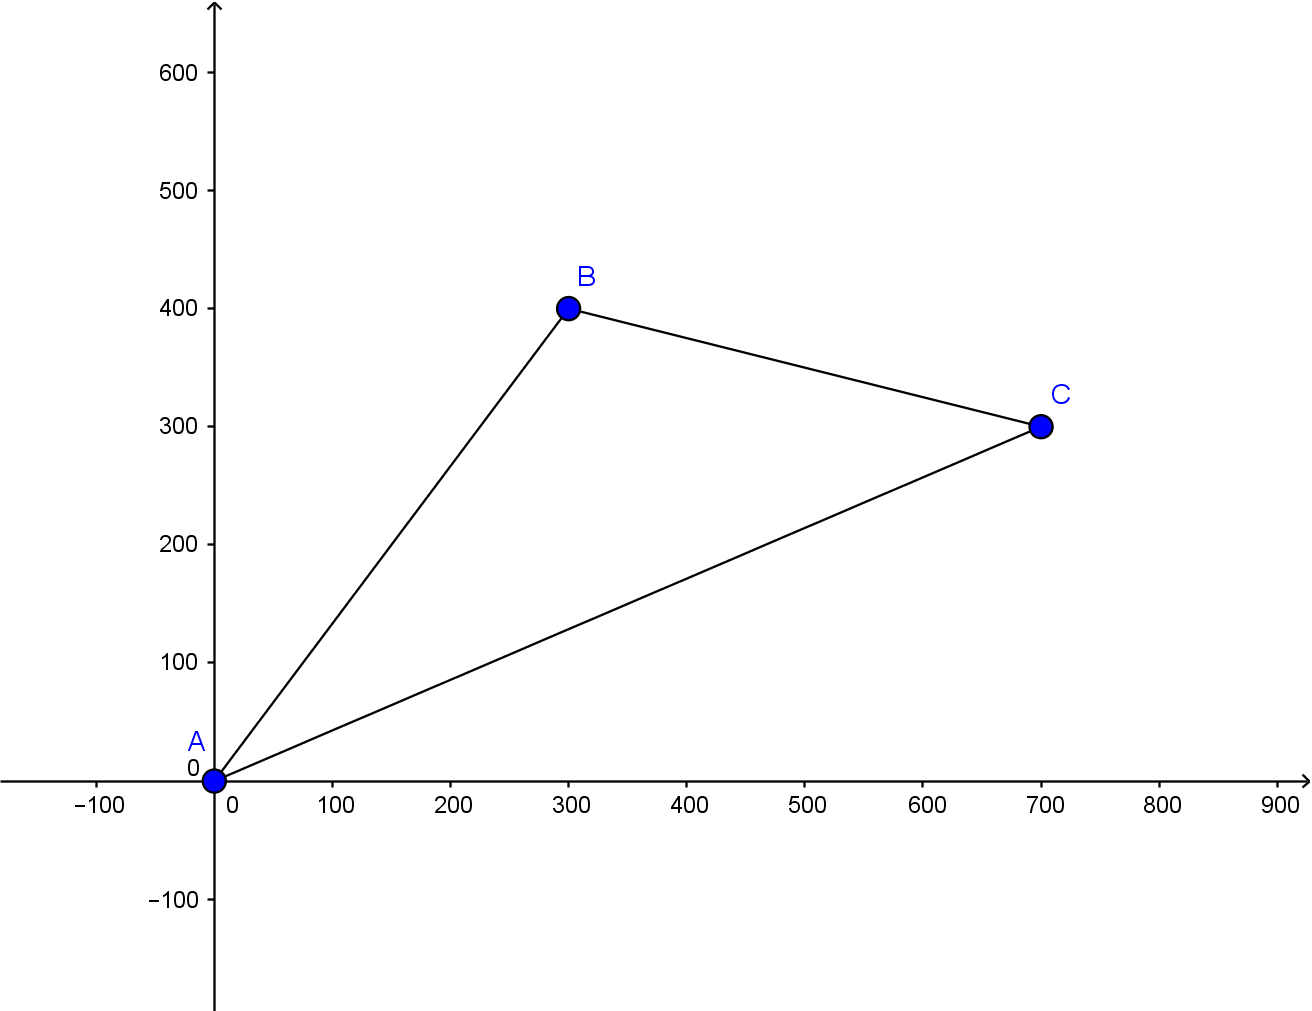
\includegraphics[width=\textwidth]{20}
\begin{equation}
  Min\ Z = \sqrt{x^2 + y^2} + \sqrt{\paren{300 - x}^2 + \paren{400 - y}^2} + \sqrt{\paren{700-x}^2 + \paren{300 - y}^2}
\end{equation}
\begin{align*}
  x,y \in \mathbb{R}
\end{align*}
\end{homeworkProblem}




\end{document}
